\Chapter{System Architecture}

\section{Overview}
This application uses HTTPS exclusively for security reason, except in local developer environment we use HTTP, as shown in Figure ~\ref{fig:deployment}.

\vspace{3em}
\begin{figure}[H]
\begin{center}
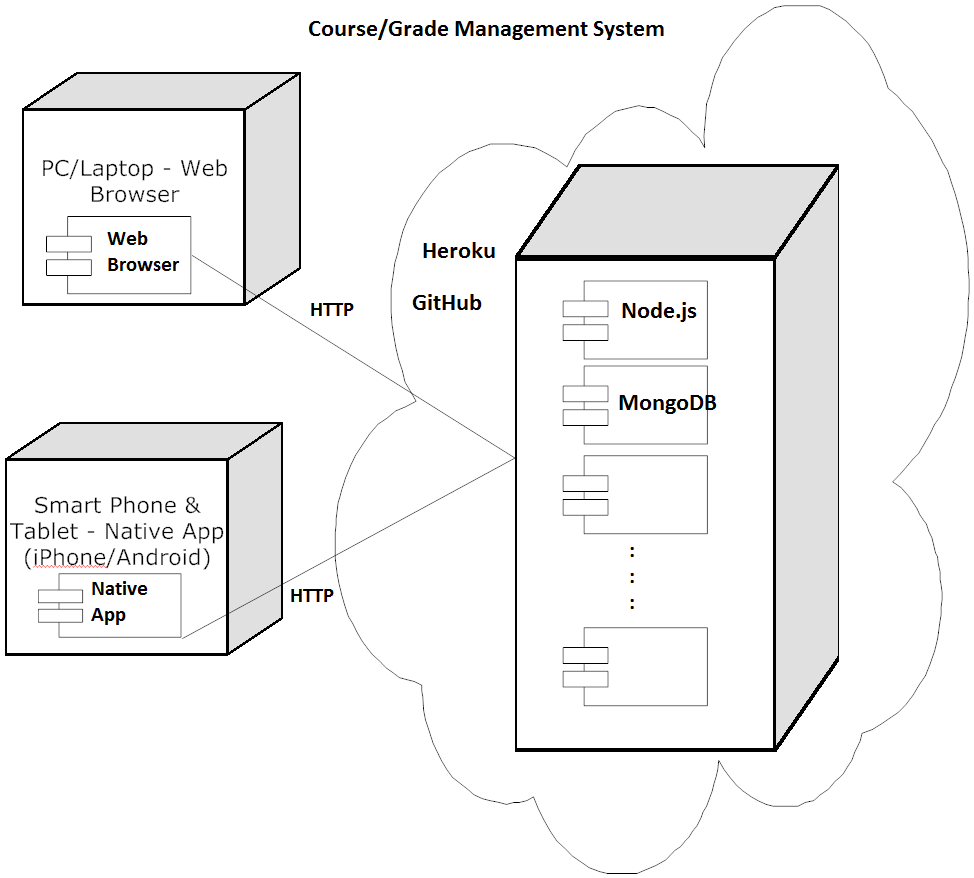
\includegraphics[height=3.8in,width=6.5in]{images/deployment.png}
\caption{Deployment Diagram}
\label{fig:deployment}
\end{center}
\end{figure}

\section{Deployment Workflow}
There are three type of environments used in the deployment workflow: Development, Staging and Production. And this is how the workflow will look like in Figure  ~\ref{fig:system-integration}.

\vspace{3em}
\begin{figure}[H]
\begin{center}
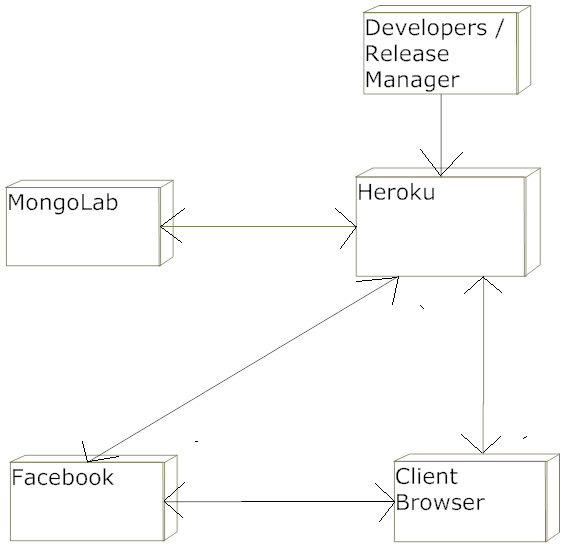
\includegraphics[height=3.8in,width=6.5in]{images/systemIntegration.png}
\caption{System Integration}
\label{fig:system-integration}
\end{center}
\end{figure}

\begin{itemize}
\item Developers work on new features or bugs fixing in development branch. Only minor updates are committed directly to stable development branch.
\item Once features are implemented and/or set of bugs are fixed, they are merged in to staging branch and deployed to staging environment for testing and quality assurance
\item After testing is completed, the snapshop of staging branch is kept for prduction deployment, otherwise the process will repeat until the testing is completed.
\item On the release date, the working staging branch is deployed to production environment.
\end{itemize}

On this project, git is used as code repositories, to manage developments, staging and production branch. And Heroku toolbelt is also used to set the enviroment config variable for each deployment. Heroku allows users to use git to deploy automatically from local repositories. 
 
\section{Heroku}
In this project there are two sets of heroku instance used, staging and production. 
Heroku connects to MongoLab using Mongo Protocol to get and/or write the data to database, and Heroku also talks to Facebook server via Open Graph API.

\section{MongoLab}
In this project there are three sets of mongo database used, development, staging and production. It is important to keep the versions of database since new version of changes may include changes in database structure, so rolling back or forward the application version would not cause any error. 

\section{Facebook}
Facebook is playing an important role in this project. Facebook provides user authentication and social media integration. Facebook allows connection using Facebook API and Open Graph API.

\section{Client Browser}
Client browser uses HTTPS GET for static content, and HTTPS POST for AJAX request to Heroku. And client browser also connects to Facebook server directly using Facebook API and Open Graph API in HTTPS.
 
